\documentclass{../../myassignment}

\courselabel{IN1080}
\exercisesheet{Assignment 1}{Measuring Voltages}
\student{Rolf Vidar Hoksaas with Jonatan H. Hansen}

\newcommand{\ohm}{$\Omega$ }
\newcommand{\volt}{$V$ }
\newcommand{\amperes}{$A$ }
\newcommand{\percent}{$\%$}
\newcommand{\micro}{$\mu$}
\newcommand{\kilo}{$k$}

\begin{document}
	1)
	\begin{answer}
		46.4 \ohm at the RS-12 multimetre
	\end{answer}

	2)
	\begin{answer}
		46.4 \ohm at the NI elvis digital multimetre
	\end{answer}

	3)
	\begin{answer}
		1.28 \percent
	\end{answer}

	4)
	\begin{answer}
		4.93 \volt
	\end{answer}

	5)
	\begin{answer}
		4.92 \volt	
	\end{answer}

	6)
	\begin{answer}
		0.20 \percent
	\end{answer}

	7)
	\begin{answer}
		5.0055 \volt
	\end{answer}

	8)
	\begin{answer}
		5.0083 \volt
	\end{answer}

	9)

	\begin{answer}
		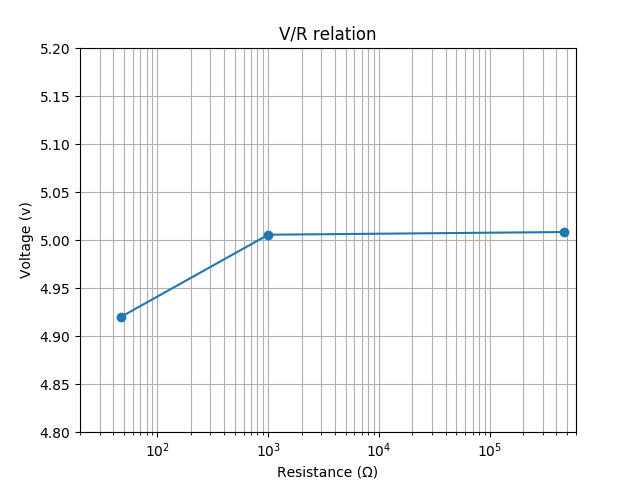
\includegraphics[scale=0.9]{relvoltohm.png}
	\end{answer}

	10)
	\begin{answer}
		9 \micro\amperes
	\end{answer}

	11)

	\begin{answer}
		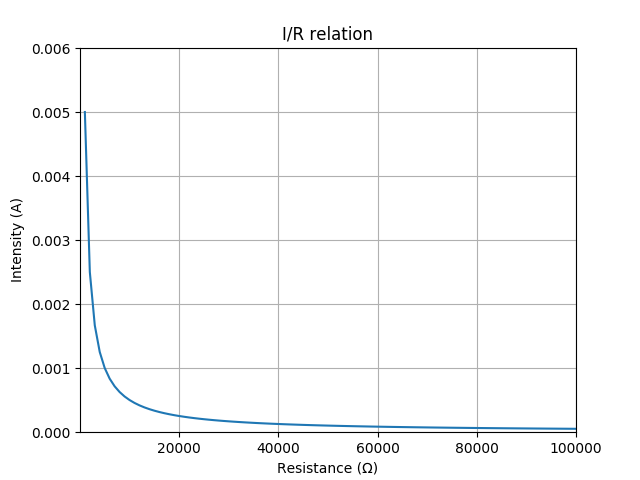
\includegraphics[scale=0.8]{relampereohm.png}
	\end{answer}


	12)
	\begin{answer}
		19 \kilo\ohm %  V_s = 100 * R_s) / (R_s + R_l), V_l = I_l * R_l = 5mA * 1kOhm = 5 V, V_s = 100 - 5 = 95 V. 95 V = I_s * R_s; R_s = 95/0.005 = 19
	\end{answer}

	13)

	\begin{answer}
		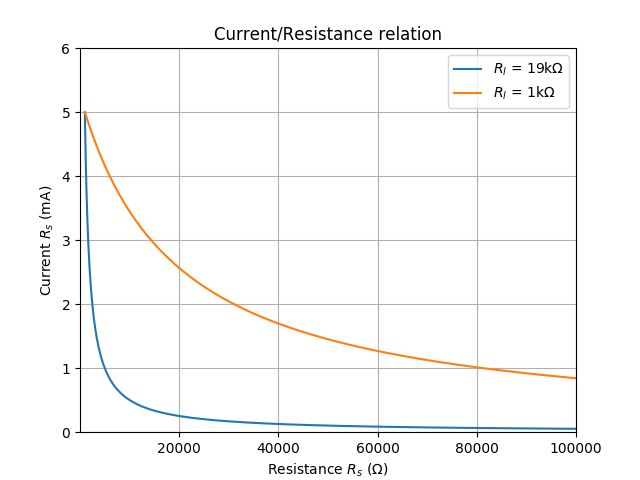
\includegraphics[scale=0.8]{variableresistor.png}
	\end{answer}

	14)
	
	\begin{answer}
		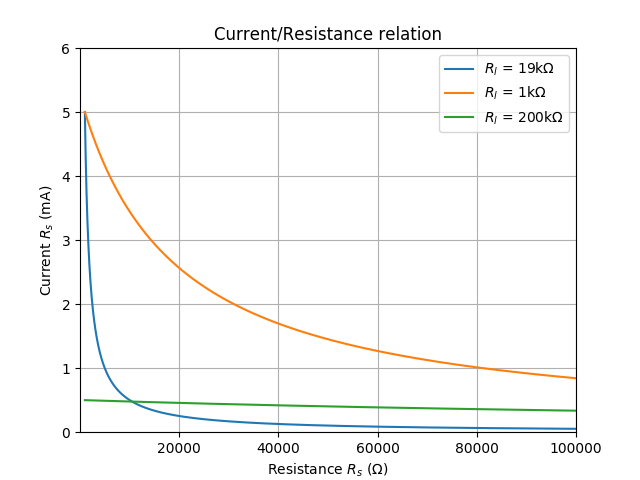
\includegraphics[scale=0.8]{bigvariableresistor.png}
	\end{answer}


\end{document}


